\documentclass[tikz]{standalone}
%tikz package already loaded by 'tikz' option
\usetikzlibrary{shapes,fit,backgrounds}

\begin{document}

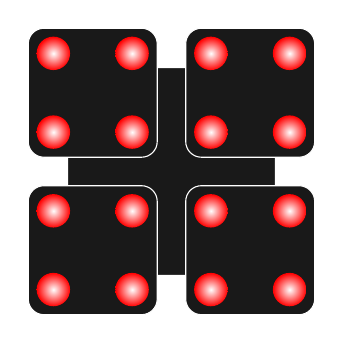
\begin{tikzpicture}[
		led/.style={
			circle,outer color=red,inner color=white,shading=radial,inner sep=1.5mm,
		},
		panel/.style={
			draw=white!90,fill=black!90,inner sep=1mm,rounded corners=2mm,
		},
	]

	% 4 red dots in each matrix
	\foreach \x in {0,...,3}
	\foreach \y in {0,...,3}
	\node [led] at (\x,\y) (dot-\x-\y) {};

	\begin{scope}[on background layer]
		% background panel connecting all four main panels
		\node[panel,inner sep=6mm,fit=(dot-1-1) (dot-1-2) (dot-2-1) (dot-2-2)] {};

		\node[panel,fit=(dot-0-0) (dot-0-1) (dot-1-0) (dot-1-1)] {};
		\node[panel,fit=(dot-0-2) (dot-0-3) (dot-1-2) (dot-1-3)] {};
		\node[panel,fit=(dot-2-0) (dot-2-1) (dot-3-0) (dot-3-1)] {};
		\node[panel,fit=(dot-2-2) (dot-2-3) (dot-3-2) (dot-3-3)] {};

	\end{scope}

\end{tikzpicture}

\end{document}
